\documentclass[]{article}
\usepackage{amsmath}
\usepackage[margin=0.8in]{geometry}
\usepackage{graphicx}
\usepackage{grffile}
\usepackage{graphics}
\usepackage{amssymb}% http://ctan.org/pkg/amssymb
\usepackage{pifont}% http://ctan.org/pkg/pifont
\newcommand{\cmark}{\ding{51}}%
\newcommand{\xmark}{\ding{55}}%
\graphicspath{ {images/} }
%opening
\title{NWEN 242 Assignment3}
\author{Yongbo Yu ||ID:300390526
}
\usepackage{amsmath}
\usepackage[margin=0.8in]{geometry}
\begin{document}
\maketitle
\section*{Q1}
\subsection*{a}
Pipelined:Cycle time determined by the slowest stage : 350ps\newline
Single-cycle: Cycle time determined by sum of all stages : 1250ps\newline
\subsection*{b}
LW instruction uses all the five stages \newline
Pipelined processor takes 5 cycles at 350ps per cycle for total latency of 1750ps.\newline
Single-cycle processor takes (250+350+150+300+200)=1250ps.\newline
\subsection*{c}
Data memory is utilized only by LW and SW instructions. So the utilization is 35\% of the clock cycles.

\subsection*{d}
The utilization for this part is determined by R-type instructions and LW instructions.The utilization is 65\%.  
\subsection*{e}
CPI for Muti-cycle machine =45\% $\times$ 4 + 20\% $\times 5 $+ 15\% $\times$ 4 = 4\newline
\begin{center}
	\begin{tabular}{c c c c c }
		&Single-cycle &Multi-cycle & Pipeline \\
		Cycle time&1250ps&350ps&350ps\\
	     CPI&1&4&1\\
	     Excution time &3.6&4&1\\
		
	\end{tabular}
	
\end{center}

\section*{Q2}
\subsection*{a}
firstly we assume write first then read. \newline
\newline
add r5,r2,r1 \newline
nop\newline
nop\newline
lw r3,4(r5)\newline
lw r2,0(r2)\newline
nop\newline
or r3,r5,r3\newline
nop\newline
nop\newline
sw r3.0(r5)\newline

\subsection*{b}
We can't have any performance gain by reordering these instructions. Because no matter how we rearrange the code there always has at least five "nop".\newline
\subsection*{c}
Yes, we still need to insert nops to ensure correct execution.  With forwarding we only reduce the cycle bubbles. But we still need use 1 cycle bubble between lw and R-type to make the code work correctly. 
\section*{Q3}
\subsection*{a}
I assume write first then read.\newline
lw \$t1, 4(\$t2)\newline
nop\newline
lw \$t2 ,4(\$t1)\newline
nop\newline
add \$t3,\$t1, \$t2\newline
sw \$t3, 8(\$t1)\newline
lw \$t4, 12(\$t0)\newline
nop\newline
add \$t5, \$t1,\$t4\newline
sw \$t5, 16(\$t2)\newline
\subsection*{b}
lw \$t1, 4(\$t2)\newline
lw \$t4, 12(\$t0)\newline
lw \$t2 ,4(\$t1)\newline
add \$t5, \$t1,\$t4\newline
add \$t3,\$t1, \$t2\newline
sw \$t5, 16(\$t2)\newline
sw \$t3, 8(\$t1)\newline

After reordering the code, we don't need to insert nop to make the code works correctly, which will improve the performance. \newline

\subsection*{c}
lw  \$t4, 12(\$t0) \newline
add \$t5, \$t1, \$t4 \newline
sw  \$t5, 16(\$t2) \newline
MEM/WB.RegisterRd=ID/EX.RegisterRs \newline
EX/MEM.RegisterRd=ID/EX.RegisterRd\newline




\section*{Q4}
\subsection*{a}
16: lw \$t2, 4(\$t1)\newline
20: beq \$t2, \$t1, 10\newline
...\newline
xx: sw \$t2, 16(\$t2)\newline
 xx should be 64. Because as the instruction branch equal be executed then index become 24. Then as it shown above the offset is 10. Then xx= 10*4+24=64. \newline
\subsection*{b}
16: lw \$t2, 4(\$t1)\newline
20: beq \$t2, \$t1, 10\newline
24:nop\newline
28:nop\newline
Because we want the result from the beq instruction. But we can only have the result after the code fully executed which means we need to put ten nops between beq instruction and the next instruction. \newline
\subsection*{c}
lw \$t2, 4(\$t1) \newline
beq \$t2, \$t1, 10\newline
nop\newline
sw \$t2, 16(\$t2)\newline
With extra memory and fully forwarding we only need to insert one nop between beq and sw.\newline
\section*{Q5}
\subsection*{a}
\begin{center}
	\begin{tabular}{c c c c c c c}
		&T & NT & T & T & NT \\
        &\cmark&\xmark&\xmark&\cmark&\xmark\\
       T&T & NT & T & T & NT\\
        	
	\end{tabular}

\end{center}
From the table we can find the accuracy for always-taken is $\frac{2}{5}$=40\%\newline
\begin{center}
	\begin{tabular}{c c c c c c c}
		&T & NT & T & T & NT \\
		&\xmark& \xmark &\xmark&\cmark &\xmark\\
	 NT &T & NT & T & T & NT\\		
	\end{tabular}
\end{center}
The accuracy for always-not-taken is $\frac{3}{5}$=20\%\newline
\subsection*{b}
\begin{center}
	\includegraphics[width=60mm,scale=0.5]{1.jpg}
\end{center}
The accuracy of always-taken is 60\% \newline
\begin{center}
	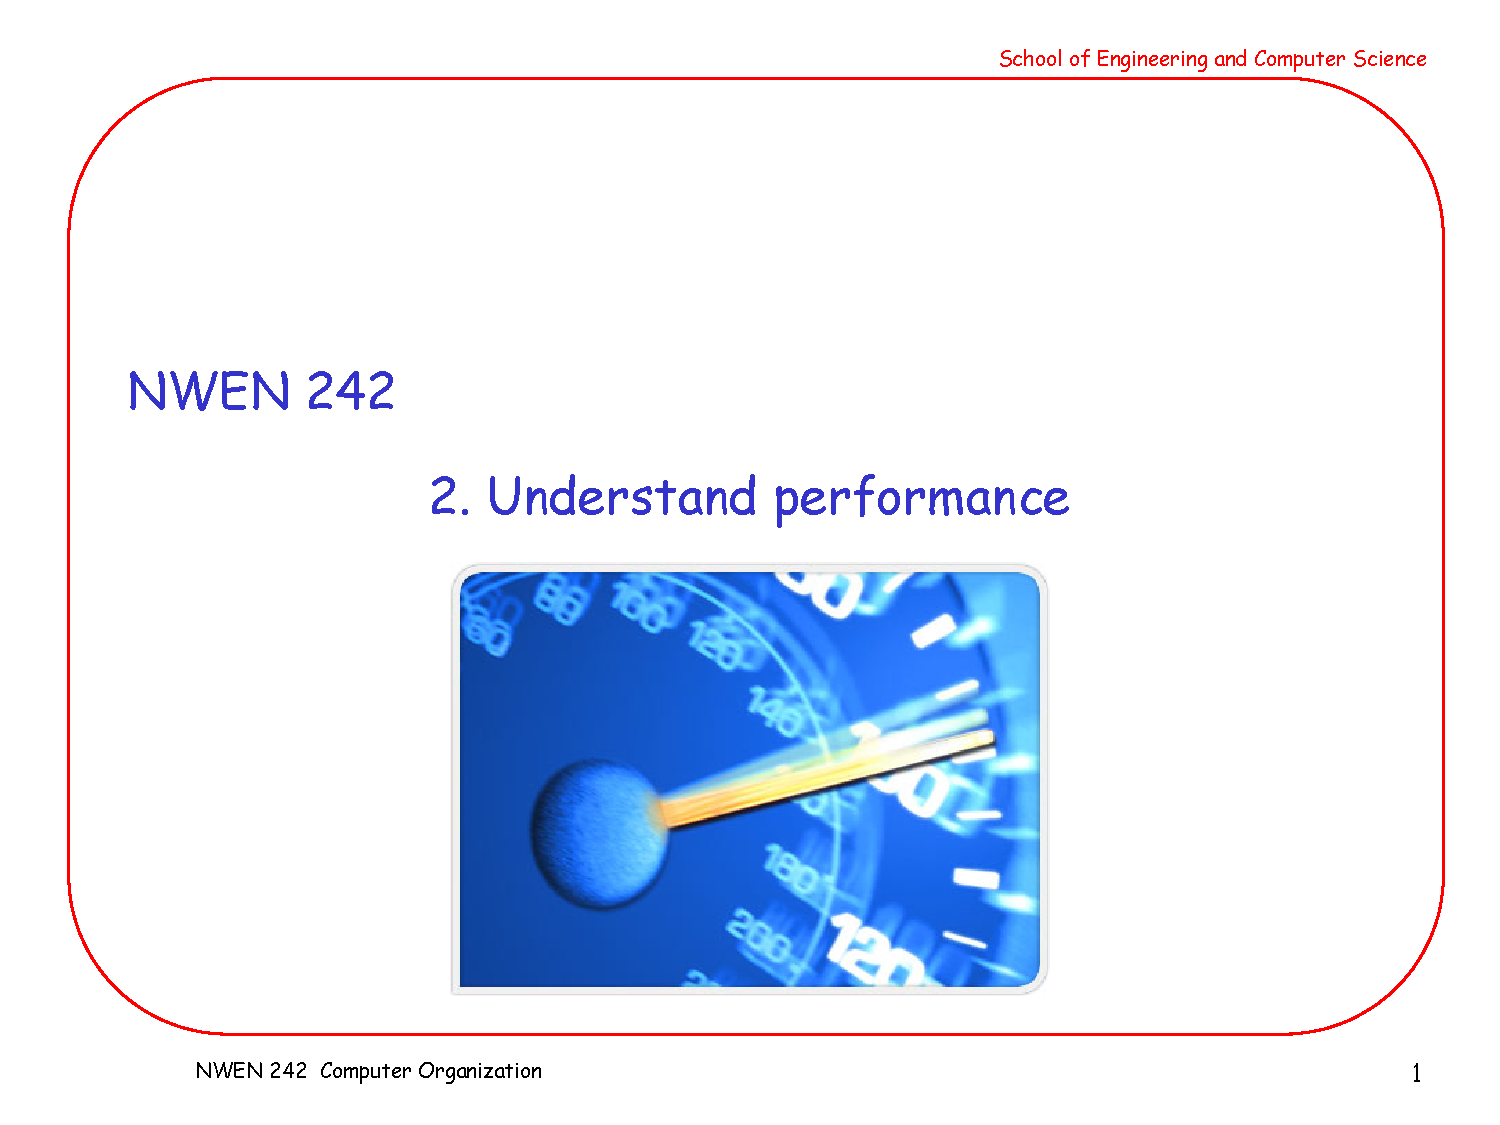
\includegraphics[width=60mm,scale=0.5]{2.jpg}
\end{center}
The accuracy of always-not-taken is 40\% \newline
\subsection*{c}


\end{document}